
\documentclass{beamer}
\usecolortheme{dove}
\setbeamertemplate{navigation symbols}{}
\usepackage{amsmath,amssymb,amsfonts,amsthm, multicol, subfigure, color}
\usepackage{bm}
\usepackage{graphicx}
\usepackage{tabularx}
\usepackage{booktabs}
\usepackage{hyperref}
\usepackage{pdfpages}
\usepackage{xcolor}
\definecolor{seagreen}{RGB}{46, 139, 87}
\def\independenT#1#2{\mathrel{\rlap{$#1#2$}\mkern2mu{#1#2}}}
\newcommand\indep{\protect\mathpalette{\protect\independenT}{\perp}}
\def\log{\text{log}}
\newcommand\logit{\text{logit}}
\newcommand\iid{\stackrel{\text{iid}}{\sim}}
\newcommand\E{\text{E}}
\newcommand\V{\text{V}}
\renewcommand\P{\text{P}}
\newcommand{\Cov}{\text{Cov}}
\newcommand{\Cor}{\text{Cor}}
\newcommand\doop{\texttt{do}}
\usepackage{stackrel}
\usepackage{tikz}
\usetikzlibrary{arrows,shapes.arrows,positioning,shapes,patterns,calc}
\newcommand\slideref[1]{\vskip .1cm \tiny \textcolor{gray}{{#1}}}
\newcommand\red[1]{\color{red}#1}
\newcommand\blue[1]{\color{blue}#1}
\newcommand\gray[1]{\color{gray}#1}
\newcommand\seagreen[1]{\color{seagreen}#1}
\newcommand\purple[1]{\color{purple}#1}
\newcommand\orange[1]{\color{orange}#1}
\newcommand\black[1]{\color{black}#1}
\newcommand\white[1]{\color{white}#1}
\newcommand\teal[1]{\color{teal}#1}
\newcommand\magenta[1]{\color{magenta}#1}
\newcommand\Fuchsia[1]{\color{Fuchsia}#1}
\newcommand\BlueGreen[1]{\color{BlueGreen}#1}
\newcommand\bblue[1]{\textcolor{blue}{\textbf{#1}}}
\newcommand\bred[1]{\textcolor{red}{\textbf{#1}}}
\newcommand\bgray[1]{\textcolor{gray}{\textbf{#1}}}
\newcommand\bgreen[1]{\textcolor{seagreen}{\textbf{#1}}}
\newcommand\bref[2]{\href{#1}{\color{blue}{#2}}}
\colorlet{lightgray}{gray!40}
\pgfdeclarelayer{bg}    % declare background layer for tikz
\pgfsetlayers{bg,main} % order layers for tikz
\newcommand\mycite[1]{\begin{scriptsize}\textcolor{darkgray}{(#1)}\end{scriptsize}}
\newcommand{\tcframe}{\frame{
%\small{
\only<1|handout:0>{\tableofcontents}
\only<2|handout:1>{\tableofcontents[currentsubsection]}}
%}
}

\newcommand{\goalsframe}{\begin{frame}{Learning goals for today}
By the end of class, you will be able to
\begin{itemize}
    \item use statistical learning to estimate when data are sparse
    \item work with models that are ``wrong''
 \end{itemize} 
  \vskip .2in
\end{frame}}

\newcommand{\credible}{\begin{frame}{Credible science}
\begin{enumerate}
\item replicability
\item reproducibility
\end{enumerate}
\end{frame}}

\usepackage[round]{natbib}
\bibliographystyle{humannat-mod}
\setbeamertemplate{enumerate items}[default]
\usepackage{mathtools}

\title{Studying Social Inequality with Data Science}
\author{Ian Lundberg}
\date{\today}

\begin{document}

\begin{frame}
\begin{tikzpicture}[x = \textwidth, y = \textheight]
\node at (0,0) {};
\node at (1,1) {};
\node[anchor = north west, align = left, font = \huge] at (0,.9) {Studying\\Social Inequality\\with Data Science};
\node[anchor = north east, align = right] (number) at (1,.9) {INFO 3370 / 5371\\Spring 2024};
\node[anchor = north, font = \Large, align = center] at (.5,.5) {Statistical Learning};
\end{tikzpicture}
\end{frame}

\goalsframe

\section{Some statistical learners}

\begin{frame}
\huge some statistical learning algorithms
\end{frame}

\begin{frame}{Ordinary Least Squares}

$\hat{Y}_i = \hat\alpha + \hat\beta X_i$ with $\hat\alpha$ and $\hat\beta$ chosen to minimize
$\underbrace{\sum_{i=1}^n \left(Y_i - \hat{Y}_i\right)^2}_\text{Squared Error}$ \vskip .2in
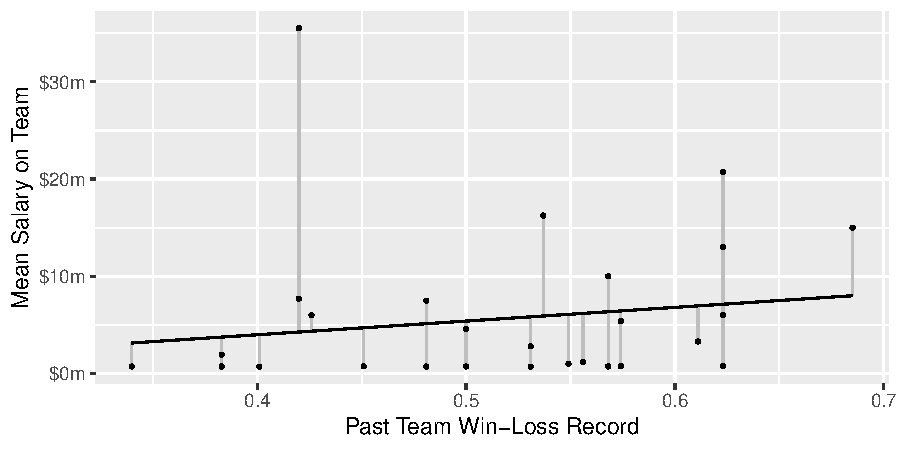
\includegraphics[width = \textwidth]{illustrate_ols}

\end{frame}

\begin{frame}{Penalized regression}

$\hat{Y}_i = \hat\alpha + \hat\beta X_i$ with $\hat\alpha$ and $\hat\beta$ chosen to minimize
$$\underbrace{\sum_{i=1}^n \left(Y_i - \hat{Y}_i\right)^2}_\text{Squared Error} + \underbrace{\lambda\beta^2}_\text{Penalty}$$ \vskip .1in
\includegraphics<2>[width = \textwidth]{ridge_comparison_1}
\includegraphics<3>[width = \textwidth]{ridge_comparison_2}
\includegraphics<4>[width = \textwidth]{ridge_comparison_3}
\end{frame}

\begin{frame}
\begin{tabular}{ll}
ols regression & standard tool \\
penalized regression & OLS with reduced variance
\end{tabular}
\end{frame}

\begin{frame}{Splines}

Regression with some terms estimated locally\\in regions of the data separated by \textbf{knots} \vskip .2in

\includegraphics<1>[width = \textwidth]{linear_spline}
\includegraphics<2>[width = \textwidth]{quadratic_spline}
\includegraphics<3>[width = \textwidth]{cubic_spline}

\end{frame}

\begin{frame}
\begin{tabular}{ll}
ols regression & standard tool \\
penalized regression & OLS with reduced variance \\
splines & capture smooth nonlinearity
\end{tabular}
\end{frame}

\begin{frame}{Decision tree}

Assume the response is locally flat\\Find places where it jumps \vskip .2in

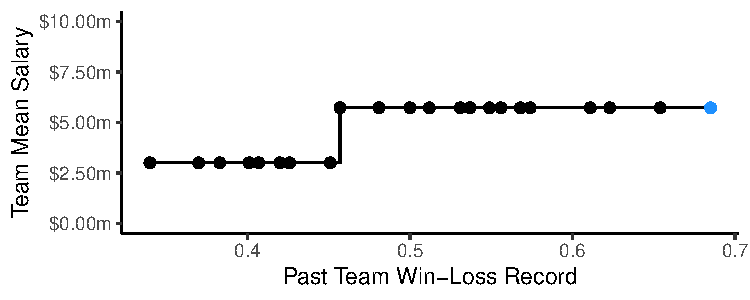
\includegraphics[width = \textwidth]{tree}

\end{frame}

\begin{frame}
\begin{tabular}{ll}
ols regression & standard tool \\
penalized regression & OLS with reduced variance \\
splines & capture smooth nonlinearity \\
trees & capture discrete nonlinearity
\end{tabular}
\end{frame}


\goalsframe

\end{document}
